\question[4]
Gib für den abgebildeten Graphen die Implementierung in Python als Adjazenzmatrix an.
Die Knoten a,b,c,.. sind auf die Indizes 0,1,2,... abgebildet.

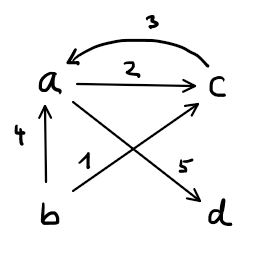
\includegraphics[height=4cm]{\pfad/Graphen/Aufgaben/adjazenzmatrix_05a/adjazenzmatrix_05a.png}
\begin{solutionbox}{5cm}
\begin{lstlisting}
inf = float('inf')
G = [[0,inf,2,5],
     [4,0,1,inf],
     [3,inf,0,inf],
     [inf,inf,inf,0]]

\end{lstlisting}
\end{solutionbox}
